A percepção automática ou visão computacional feita por computadores, se vale do processamento digital de imagens para simular a visão humana, incluindo o aprendizado e a capacidade de fazer inferências, assim como, agir com base nas informações adquiridas. 

Por sua vez, o processamento digital de imagens executa operações matemáticas em imagens digitais em domínios diferentes, é utilizado, de maneira geral, para melhorar imagens para percepção humana, e, como é abordado no presente trabalho, com enfoque computacional, a fim de armazená-las em um espaço com melhor alocação, transmití-las com maior velocidade e/ou representá-las com maior desempenho. 

De maneira a simplificar o estudo do processamento digital de imagens, \citeonline{Gonzalez}, dividiram os processos digitais em três tipos de operações. São listadas as operações de baixo nível, de médio nível e de alto nível, como seguem:

\begin{enumerate}
\item operações de baixo nível englobam operações primitivas, como  pré-processamento de imagens, como melhorar contraste, brilho, assim como, aguçamento de imagens e redução de ruídos. Geralmente possuem como entrada a imagem original e como saída a imagem tratada;

\item nas operações de médio nível, regiões ou objetos são identificados descrevendo-os individualmente, de modo, a classificá-los ou reconhecê-los, sem considerar em que contexto essas regiões sem enquadram. Como imagem de entrada para essas operações pode-se usar a imagem original, porém, é mais comum o uso de imagens previamente tratadas com operações de baixo nível. Após o processamento, essas operações retornam atributos dessa imagem, como, regiões, contornos e bordas;

\item já as operações de alto nível pretendem vincular ou inferir a um conjunto de objetos reconhecidos um determinado contexto. As entradas desses tipos de operações variam, porém, de maneira geral, descritores são utilizados. Após encontradas todas as regiões e objetos é possível identificar em qual contexto estão inseridos. 

\end{enumerate}

Para entender melhor como o processamento digital de imagens funciona, convém iniciar pelo menor elemento em um dispositivo de exibição/aquisição, o pixel\footnote{pixel - Contração do inglês: "Picture Element"}, ao qual é possível atribuir-se uma propriedade, comumente uma cor, ou como será visto, uma intensidade. De uma forma mais simples, um pixel é o menor ponto que forma uma imagem digital, sendo que o conjunto de pixels forma a imagem inteira.

Uma imagem pode ser definida como sendo a representação visual de um objeto. Do ponto de vista matemático, uma imagem é considerada uma função bidimensional f(x,y) onde x e y são coordenadas planas, e a amplitude de f em qualquer par de coordenadas (x,y) é chamada de intensidade ou nível de cinza da imagem no referido ponto. Quando (x,y) e a amplitude fazem parte de um conjunto de valores finitos ou discretos, a imagem é chamada de imagem digital \cite {Gonzalez}. 

Em outras palavras, uma imagem digital pode ser representada através de uma matriz nxm, onde, n é a resolução horizontal da captura e m é a resolução vertical da captura, cada elemento da matriz corresponde à intensidade ou nível de cinza f(x,y) em um determinado ponto da imagem. Para imagens binárias (em preto e branco) os valores dos pixels podem assumir os valores 0 e 1. Para imagens em tons de cinza esses valores podem variar de 0 a 255 e, finalmente, para imagens coloridas, tem-se que o valor do pixel é representado por três valores variando de 0 a 255 cada um, no modelo de cores RGB.


\section{Processamento de imagens coloridas}


Para entender como os descritores de cor são utilizados, é necessário definir previamente o conceito de cor e listar algumas de suas características. A cor pode ser definida como um fenômeno perceptual da luz quando incide e é refletida por um objeto \cite {Gonzalez}. Como se pode observar, o conceito de cor é diretamente relacionado ao conceito de luz \cite {Gonzalez}. Portanto, ao se referir ao conceito de cor deve-se mencionar, obrigatoriamente, a luz.

Dois conceitos preliminares são particularmente importantes para o entendimento do conceito de percepção de cor. São eles: a luminância e a crominância. A luminância contém a informação da quantidade das cores pretas e brancas presentes em uma imagem. O cérebro humano interpreta essa informação como a quantidade de cinza presente na cor (ou brilho). A crominância informa a respeito da tonalidade de uma cor. É a frequência dominante do raio de luz. A combinação destes dois conceitos, em diferentes proporções, permite ao cérebro perceber o espectro de cores visível em uma determinada imagem ou cena. Para representar as cores existem modelos ou sistemas de cores \cite {Gonzalez}, como por exemplo RGB (“red, green, blue”), CMY (“cyan, magenta, yellow”),HSV (“matiz, saturação, intensidade”), YIQ (luminância, em-fase, quadratura) e LAB (luminosidade, verde-vermelho, azul-amarelo).

O sistema Red, Green, Blue é um sistema de representação de cor aditivo \cite{Bimbo} e se baseia na teoria dos três estímulos proposta por \citeonline{Young}. Segundo essa teoria, o olho humano percebe a cor através do estímulo de três pigmentos visuais presentes nos cones da retina, que possuem sensibilidades para alguns comprimentos de onda, como por exemplo, 630 nanômetros (vermelho – red), 530 nanômetros (verde – green) e 450 nanômetros (azul – blue). Uma representação desse sistema pode ser formulada através de um cubo com os eixos R, G e B. Podemos dizer que a origem representa a cor preta, os vértices das coordenadas (1, 1, 1) representam o branco, os vértices que estão sobre os eixos representam as cores primárias e os vértices restantes representam os complementos das primárias. 

É importante observar que cada ponto no interior do cubo corresponde a uma cor, representada por uma tripla (R, G, B), com os valores de R, G e B variando de 0 a 1. Os tons de cinza são representados ao longo da diagonal principal do cubo, que se inicia no ponto de origem até o vértice que foi apontado como a cor branca. Portanto, é possível, afirmar que cada tom de cinza presente no cubo é formado por contribuições iguais das cores primárias que o compõem. 


\section{Baixo Nível - Filtros}

Os processos de visão computacional, muitas vezes, necessitam de uma etapa de pré-processamento envolvendo o processamento de imagens. As imagens de onde queremos extrair alguma informação em certos casos precisam ser convertidas para um determinado formato ou tamanho e precisam ainda ser filtradas para remover ruídos provenientes do processo de aquisição da imagem. \cite{Gonzalez}

Nessa concepção, ruídos podem aparecer de diversas fontes, como por exemplo, o tipo de sensor utilizado, a iluminação do ambiente, as condições climáticas no momento da aquisição da imagem, a posição relativa entre o objeto de interesse e a câmera. Note que ruído não é apenas interferência no sinal de captura da imagem, mas também interferências que possam atrapalhar a interpretação ou o reconhecimento de objetos na imagem. Os filtros aparecem como ferramentas básicas, para remover ruídos de imagens.

No domínio espacial, plano que contém os pixels de uma imagem, a aplicação de filtros se limita à alteração direta dos pixels ou em sua vizinhança, de forma que, a uma janela é movida pixel a pixel na imagem de entrada para gerar uma imagem de saída.

\subsection{Transformações de intensidade}

As transformações de intensidade estão entre as técnicas mais simples de processamento digital de imagens, nessas transformações uma função matemática de transformação é aplicada no nível de intensidade dos pixels. Exemplos básicos incluem transformações logarítmicas, polinomiais de n-ésima potência e de negativo. Em uma transformação de negativo, a ser utilizada na identificação das linhas de campo, a intensidade dos pixels é revertida segundo a expressão \cite{Gonzalez}:

\begin{equation}
	S = L-1-E 
\end{equation}

Onde S representa o valor do pixel depois do processamento, (L-1) é o limite máximo de nível de intensidade dos pixels da imagem original e E o valor do pixel original antes do processamento.

Na verdade, o objetivo dessa expressão é reverter a intensidade de todos os pixels da imagem, de forma a se obter algo semelhante a um negativo fotográfico, de modo que a imagem resultante se torne mais adequada para a aplicação do que a original.

\subsection{Histogramas}

Histograma é a representação de um conjunto de dados previamente tabulados e divididos em classes uniformes. Na estatística, um histograma é uma representação gráfica da distribuição de frequências de uma massa de medições \cite{Wand}. Quando o número de dados aumenta indefinidamente e o intervalo de classe tende a zero, a distribuição de frequência passa para uma distribuição de densidade de probabilidades \cite{Wand}. A construção de histogramas tem caráter preliminar em qualquer estudo e é um importante indicador da distribuição de dados. Pode indicar se uma distribuição aproxima-se de uma função normal, como pode indicar mistura de populações quando se apresentam bimodais. \cite{Wand}

Em processamento de imagens é usado de forma geral para se obter estatísticas espaciais úteis da imagem \cite{Gonzalez}. Algumas aplicações do histograma de uma imagem digital incluem, mas não se limitam, a da probabilidade de ocorrência, de intensidades de pixels, de cores e de gradientes. Após sua normalização, a soma de todas as probabilidades de um determinado histograma é 1. 

Umas das mais conceituadas formas de realçar uma imagem é equalizando seu histograma de cores ou de intensidades \cite{Gonzalez}. Essa equalização procede gerando uma função de transformação que busca produzir uma imagem de saída que tenha um histograma uniforme. O histograma de cores pode representar a distribuição global de cores completa da imagem ou de apenas uma determinada parte da mesma.
E, como veremos nos próximos capítulos, o histograma de gradientes normalizado pode ser utilizado para extrair informações importantes sobre o formato de objetos presentes em uma determinada imagem identificando transições de borda e mostrando sua magnitude.

Histogramas de contraste e de brilho podem dizer se a imagem foi exposta corretamente, já os de luminância levam em consideração que o olho humano é mais sensível a certos tipos de cores que a outros. No histograma de luminância cada pixel é convertido de modo a representar a luminosidade. Isso é feito baseado em uma média com pesos diferentes para cada uma das cores em cada pixel \cite{Wand}. Esses pesos assumem que o verde representa 59\% da luminosidade percebida, enquanto que o vermelho e o azul representam apenas 30\% e 11\%, respectivamente. Uma vez que cada pixel foi convertido em luminosidade, um histograma de luminância é produzido ao se contar quantos pixels estão em cada valor de luminância, ou seja, são produzidos da mesma forma que histogramas de cores apenas substituindo as cores por luminâncias.


 
\subsection{Filtros Espaciais}

Em processamento digital de imagens, o termo filtro refere-se ao fato de limitar, ou permitir, a passagem de certas características ou componentes de uma imagem original para uma tratada \cite{Gonzalez}. De forma geral isso é executado usando um pixel e/ou sua vizinhança de pixels. 
A definição do tamanho da vizinhança depende do tipo de filtro, do tipo de operação e do resultado que se deseja alcançar. Valores de vizinhança comuns são de 9, 25, 49 pixels, e formatos comuns são círculos e quadrados \cite{Gonzalez}. Uma ou mais operações de filtragem podem assumir o comportamento linear ou não linear. Entre os diversos tipos de filtros existentes destacam-se os filtros de suavização, esses são utilizados para redução de pequenos detalhes da imagem antes da extração de regiões maiores. Como exemplos de filtros lineares existem os filtros de média, também chamados de filtros passa-baixa, e como exemplos de filtros não-lineares, os filtros de estatística de ordem. 

Esse último filtro tem como principal representante o filtro da mediana, no qual o valor do pixel central é substituído pela mediana de sua vizinhança, de forma que se baseia na classificação dos pixels na área de imagem coberta por essa vizinhança (máscara) \cite{Gonzalez}. Essa classificação pode ser feita por qualquer operação que classifique os pixels, como uma Gaussiana, por exemplo. O pixel central da máscara Gaussiana, torna-se o pico da Gaussiana e os pixels vizinhos são alterados segundo a curvatura da Gaussiana, (ver figura ~\ref{Fig:FiltroGaussiana}), criando coeficientes da máscara e após aplicação causando um borramento, mas, também, reduzindo regiões menores. 
Esses filtros são bastante populares, devido a seus excelentes resultados na redução de ruídos aleatórios e impulsivos.


\begin{figure}[!t]
\centering \caption{Exemplo Filtro Gaussiana.}
\includegraphics[width=5.5in]{Imagens/Filtro_Gaussiana.png}
\DeclareGraphicsExtensions.
\caption*{Fonte: Autor}
\label{Fig:FiltroGaussiana}
\end{figure}




\subsection{Segmentação}

A segmentação, em visão computacional, é o processo de dividir ou segregar uma imagem digital em duas ou mais regiões diferentes, com o objetivo de simplificar uma imagem visando facilitar a sua análise ou interpretação \cite{Gonzalez}. Os retornos esperados, como resultados do processo de segmentação, são atributos dessa imagem, como, regiões e contornos. Convém elucidar a diferença entre borda e contorno, a borda se verifica como sendo uma transição de uma parte do contorno de um objeto. A maior dificuldade é interpretar quais bordas pertencem, efetivamente, ao contorno de uma região ou objeto.

Cada um dos pixels em uma mesma região é segmentada, levando-se em consideração alguma característica ou propriedade computacional. São propriedades comuns a cor, a intensidade, a textura ou, mesmo, a continuidade \cite{Gonzalez}. 

Todas as regiões selecionadas devem possuir limiares de características que permitam sua discretização umas das outras. De acordo com \citeonline{Benallal} e \citeonline{Broggi} é possível efetuar a segmentação seguida de reconhecimento de formato em tempo real. 

\begin{figure}[!h]
\centering \caption{Segmentação do Laranja usando como entrada uma imagem no modelo de cores HSV.}
\includegraphics[width=2.5in]{Imagens/Seg_Hsv.png}
\includegraphics[width=2.5in]{Imagens/Seg.jpeg}
\DeclareGraphicsExtensions.
\caption*{Fonte: Autor}
\label{Fig:Seg}
\end{figure}

A segmentação é especialmente importante para determinar a região de interesse. Assim, esse método será usado para encontrar uma região que possua uma caracterísitica tão importante quanto a cor, como é o caso da bola laranja do domínio Robocup Kid Size.


\subsection{Morfologia Matemática}

Morfologia é o estudo da forma, sendo o estudo morfológico o estudo das estruturas dessa forma. Em linguística, morfologia é o estudo da estrutura das palavras. Em biologia, morfologia está mais diretamente relacionada à forma de um organismo, por exemplo, a forma de uma folha pode ser usada para identificar uma planta ou a forma de uma colônia de bactérias pode ser usada para identificar sua variedade.
Por outro lado, os matemáticos consideram a morfologia uma parte da teoria de conjuntos, e por consequência, denomina-se morfologia matemática como sendo um conjunto de métodos, inicialmente desenvolvidos por \citeonline{Matheron}, que tem em comum o objetivo de estudar a estrutura geométrica de um objeto ou parte dele. 

Segundo \citeonline{Dougherty}, é possível definir a morfologia digital como sendo um caminho para descrever ou analisar a forma de um objeto digital, levando-se em conta sua estrutura geométrica, baseado no fato de que uma imagem consiste em um conjunto de pixels, que podem ser reunidos em grupos, criando uma estrutura bidimensional (forma). No presente fica subentendida a referência à morfologia digital. Certas operações matemáticas, quando aplicadas em conjuntos de pixels, podem ser usadas para ressaltar aspectos específicos das formas permitindo que sejam contadas ou reconhecidas.

A base da morfologia segundo \citeonline{Gonzalez} consiste em extrair as informações relativas à geometria e à topologia de um conjunto desconhecido (no caso uma imagem) pela transformação através de outro conjunto bem definido, chamado elemento estruturante. Operações morfológicas estão divididas em binárias (aplicadas a imagens com pixels pretos ou brancos), e sobre imagens coloridas (aplicadas a imagens em tons de cinza ou, como o próprio nome diz, em imagens coloridas).

Após processamento, um objeto é considerado um conjunto matemático de pixels brancos, sendo, cada pixel, identificado pelos seus índices de linha e coluna. No caso de operações binárias, um pixel afetado por essa operação será substituído pelo seu valor oposto. Em operações executadas em imagens coloridas pode ocorrer apenas a modificação parcial do valor do pixel.

\begin{figure}[!ht]
\centering \caption{Exemplo de erosão e dilatação para um objeto circular, com elemento estruturante circular.}
\includegraphics[width=2.5in]{Imagens/Morphology.jpeg}
\DeclareGraphicsExtensions.
\caption*{Fonte: o Autor}
\label{Fig:Morfologia}
\end{figure}

As operações básicas da morfologia digital são a erosão, em que pixels que não atendem a um dado padrão são apagados da imagem, e a dilatação, em que uma pequena área relacionada a um pixel é alterada para um dado padrão. Todavia, dependendo do tipo de imagem que está sendo processada (preto e banco, tons de cinza ou colorida), a definição dessas operações muda, assim, cada tipo deve ser considerado separadamente. 

Tanto a erosão como a dilatação aparecem como forma tratamento de ruídos provenientes do ambiente, eliminando regiões e áreas não pertencentes a região de interesse, reduzindo a área de atuação dos algoritimos subsequente para detecção da bola laranja.


\section{Transformada de Hough}

Sendo uma ferramenta conceituada e de uso comum em visão computacional, a transformada de Hough é um processo matemático que detecta formas geométricas em imagens digitais. Essa técnica, desenvolvida por \citeonline{Hough}, encontra formas que podem ser paramatrizáveis em imagens digitais como linhas, círculos e elipses, mesmo em imagens com pouca visibilidade da forma ou imagens fortemente ruidosas.

Em geral, a transformada é aplicada após a imagem sofrer um pré-processamento, comumente a detecção de bordas.A transformada de Hough encontra uma relação entre o espaço de imagem e o espaço de parâmetros. Cada transição (ou borda) de uma imagem é transformada por um mapeamento para determinar sua relação no espaço de parâmetros através de um vetor. 

As posições do vetor são incrementadas e indicarão quais os parâmetros correspondentes à forma especificada, através do máximo local do acumulador. A detecção de retas foi sua primeira aplicação mas, a transformada de Hough foi modificada para possibilitar a localização de outras formas geométricas. A transformada de Hough utilizada, majoritariamente, atualmente pode ser atribuída a \citeonline{HoughCircle} e a \citeonline{FastHough}.

Hough usou a equação definida por y = a.x + b como representação paramétrica de uma linha, fato que conduziu a soluções infinitas para linhas paralelas ao eixo y, cuja solução será abordada posteriormente.
 
O algoritmo de Hough requer um acumulador de dimensão igual ao número de parâmetros desconhecidos. Por exemplo: achar segmentos de linhas usando a equação y = ax + b, requer achar dois parâmetros para cada segmento: a e b, ou seja, duas dimensões da matriz acumuladora.

Assim, usando uma matriz acumuladora A, o procedimento de Hough examina cada pixel e calcula os parâmetros da curva (equação) especificada que passa pelo pixel. 
O procedimento examina cada pixel e calcula os parâmetros da equação de reta que passa por esse pixel, incrementando a matriz acumuladora.

Caso uma imagem que não foi pré-processada com algoritmo de detecção de bordas, fato incomum na transformada de Hough, será examinado o pixel e sua vizinhança na imagem para determinar se há evidência de borda ou transição naquele pixel. Quando todos pixels tiverem sido processados, procura-se na matriz acumuladora os maiores valores. Esses valores indicam os parâmetros de prováveis linhas na imagem.

Ao procurar os máximos na matriz acumuladora, lança-se o artifício do uso de um limiar, visando encontrar uma quantidade mínima de pontos colineares. Qualquer valor da matriz acumuladora que não for superior ao limiar será ignorado. As detecções de outras formas, utilizando a transformada de Hough, usam o mesmo princípio, com a ressalva na quantidade de parâmetros da equação que será empregada, e em consequência na dimensão do acumulador.
 
\citeonline{HoughCircle} sugeriram coordenadas polares para representação de uma linha. Essa modificação manteve a quantidade de dimensões da matriz acumuladora e resolveu a limitação inicial de linhas paralelas ao eixo y. Usando esta parametrização, todo o ponto (x,y) na equação da reta satisfará a equação r= x . cos ( q ) + y . sin ( q ). Onde os parâmetros r e q são respectivamente a distância e a orientação da linha normal à reta candidata.

Cada pixel do espaço da imagem produz uma função senoidal no espaço de Hough que alimenta um histograma. Com muitas senóides, ou seja, muitas possíveis linhas, o histograma gera diversos máximos que não correspondem efetivamente às linhas. Para resolver essa dificuldade, encontra-se a maior linha da imagem e remove-se sua contribuição do histograma. Repetindo esse procedimento até o fim das linhas encontradas, encontra-se o máximo global.

Como uma forma de inferir um formato circular à bola, é usada a transformada de Hough para círculos, na implementação sugerida por \citeonline{Davies}. Essas formas são parametrizados por x, y e r, onde x e y referem-se a posição do centro e r ao raio do círculo. Agora que a matriz acumuladora têm três dimensões, é necessário reduzir a complexidade computacional da transformada de Hough. Determinar o centro e em seguida, encontrar o raio, divide o problema em duas fases distintas amenizando as dificuldades computacionais dessa técnica.

Fica definido que a normal tangente de qualquer pixel pertencente a um círculo passa pelo centro desse círculo. Calcula-se a tangente como a linha que se ajusta melhor a todos pixels de uma vizinhança pequena (usando o método mínimos-quadrado), isso permite calcular a normal e registrá-la em um histograma. Finalmente, os máximos do histograma definem os locais de centros dos possíveis círculos. 

Encontrar o raio esconde uma dificuldade prática, existem infinitos círculos que podem ter o mesmo centro. Para sobrepor essa dificuldade, alimenta-se um histograma unidimensional com a distância de cada pixel até o centro de um determinado círculo. Assim, os máximos dos histogramas correspondem aos raios dos círculos.

Há ainda, a transformada probabilística de Hough, que afirma que é suficiente computar a transformada de Hough só de uma proporção de pixels na imagem. Estes pixels são escolhidos de forma aleatória usando-se uma função de densidade de probabilidade uniforme. Essa técnica foi  proposta por \citeonline{Kiryatti}. A transformada de Hough vem para inferir o formato circular à bola segmentada por cores e com ruídos reduzidos nas etapas de erosão e dilação.

\section{Propagação da Densidade Condicional - Condensação}

O algoritmo de condensação (Propagação densidade condicional) é um algorítimo probabilístico de visão computacional, cuja aplicação principal é detectar e rastrear objetos que se movem em um ambiente desordenado. Usa como base o filtro de partículas proposto por \citeonline{Thrun} para fins de localização de robôs móveis.

O próprio algoritmo é descrito em detalhes por \citeonline{Condensation} e foi usado para rastrear determinados tipos de curvas. Um dos aspectos mais interessantes do algoritmo é que ele não é calculado em cada pixel da imagem. Em vez disso, os pixels são escolhidos ao acaso, e apenas um subconjunto dos pixels acaba sendo processado. A presença de desordem tende a produzir distribuições de probabilidades para o estado do objeto que são multi-modais e, portanto, poderiam ser mal modelados pelo filtro de Kalmman.

O uso de bordas e cores foi proposto por \citeonline{Ross} onde o rastreamento de objetos usa a informação dessas características para calcular a verossimilhança das partículas na técnica de condensação. 

Rastrear objetos envolve modelar sistemas não gaussianos e não lineares. Filtros de partículas são métodos sequenciais de Monte Carlo com base em representações de densidades de probabilidade, que são aplicados a qualquer modelo de estado.

O filtro de partículas pesa partículas com base em uma pontuação de probabilidade e, em seguida, propaga essas partículas de acordo com um modelo de movimento ou no caso da condensação uma cor ou uma característica. Assim, aproxima a distribuição a posteriori, filtrando ponderadamente um conjunto de partículas. Essa técnica assume o modelo de Markov para estimar o estado do sistema, de forma que o estado atual é condicionalmente independente dos estados passado e futuro. Assim as observações são dependentes apenas do estado atual.

Nessa técnica ocorre a criação das partículas, onde diversas partículas são distribuídas uniformemente pela imagem. Cada partícula se refere à uma possível parte do objeto a ser rastreado. Na condensação diferentemente do filtro de partículas a atualização das partículas não ocorre. A distância euclideana entre a características esperada do objeto e a presente na imagem capturada fornece o peso dessa partícula, ou seja, qual  a probabilidade dessa partícula fazer parte do objeto. No último passo uma reamostragem das partículas onde partículas pouco prováveis são descartadas, reiniciando o processo. Usando como característica a cor, o metodo de condensação pode apontar em qual região da imagem há uma concentração de pixels que pode representar probabilísticamente onde está a bola.


\section{Descritor Histograma de Gradientes Orientados (HOG) com Máquina de Vetores de Suporte (SVM)}


No cálculo vetorial, o gradiente (ou vetor gradiente) é um vetor que indica o sentido e a direção na qual obtém-se o maior incremento possível no valor de uma grandeza. Por exemplo, a variação de intensidade de luz de uma lâmpada decai em forma de gradiente conforme nos afastamos dela. Em outras palavras, existe um operador linear que se aplicado à função de intensidade dessa lâmpada produz um vetor que sempre aponta para o ponto máximo dessa função.

Em visão computacional, o principal uso dessa técnica é a detecção de borda, quanto maior for a variância dos pixels maior será a magnitude do gradiente, enquanto, o ângulo do vetor mostra em qual direção a borda se encontra. O cálculo se inicia deslizando uma janela retangular de pixels através da imagem, e para cada janela são calculados a magnitude do gradiente e o ângulo do vetor gradiente.

Calcula-se a magnitude do gradiente varrendo a imagem pixel a pixel nas direções x e y. Subtraindo o valor da esquerda, do pixel a ser calculado, com o seu valor da direita e fazendo o mesmo com o pixel de cima e de baixo, a magnitude é dada: 

\begin{equation}
 magnitude = \sqrt{(p_{x+1} - p_{x-1})^2 + (p_{y+1} - p_{y-1})^2} 
\end{equation}

Já o ângulo do gradiente é dado por:

\begin{equation}
 \hat{a}ngulo = \arctan{ \frac {(p_{x+1} - p_{x-1})^2}  {(p_{y+1} - p_{y-1})^2}} 
\end{equation}

Onde o ponto p representa a intensidade dos pixels nas coordenadas x e y. Ao usar o conceito de gradiente, mesmo pixels diferentes podem ter o mesmo vetor de gradiente, isso se torna uma vantagem, já que torna o uso de gradientes mais robusto à variação de iluminação.

Com o uso do conceito de gradiente, é possível prosseguir para a ideia sugerida por \citeonline{Dallal}, em que um histograma é usado em conjunto com os vetores de gradiente, para um detector de pessoas. O detector de pessoas proposto usa uma janela de detecção de 64 x 128 pixels e para calcular o descritor HOG uma janela de 8 x 8 pixels dentro da janela de detecção.

Assim, segundo \citeonline{Dallal}, o próximo passo é criar um histograma para a imagem inteira. Inserindo todos os vetores calculados nessa imagem e colocando-os em um histograma de 9 bytes, que vai de 0 a 180 graus. Nesse histograma, \citeonline{Dallal} usaram gradientes sem sinal, de forma que, as orientações vão apenas de 0 a 180 graus ao invés de 0 a 360. Assim, 9 bytes distribuídos em 180 graus, significam que cada byte será responsável por uma variação de 20 graus nos vetores de gradientes. A imagem é representada por um histograma, ou, em outras palavras, um único vetor de características, ao invés de muitos vetores representando pedaços menores de muitos objetos. 

A contribuição de cada vetor de gradiente para o histograma é a parte mais importante do algoritmo. Essa contribuição é dada pela magnitude do vetor. Dividindo a contribuição entre dois bytes mais próximos, é possível minimizar o problema de gradientes que estão na fronteira entre esses dois bytes. Basicamente, se um vetor estiver com ângulo 145, como bytes possíveis, o histograma terá os valores 130 e 150, assim 25 \% da contribuição desse vetor irá para o byte de 130 graus e 75\% para o byte de 150 graus.

De outra forma, se um gradiente forte estiver bem na borda de um byte, uma pequena mudança no ângulo do gradiente (que poderia anular o gradiente no próximo byte) poderia causar um grande impacto no histograma. 

Tendo como objetivo fazer o vetor de gradientes mais robusto a mudanças de iluminação, é efetuada uma normalização dividindo todos os vetores por suas respectivas magnitudes. Dividir o vetor por sua magnitude é equivalente a normalizá-lo com tamanho máximo igual a um. Normalizar um vetor afeta apenas sua magnitude e não sua orientação.
Na verdade, ao invés de normalizar cada vetor, ou mesmo cada histograma, a normalização ocorre em blocos. Cada histograma é normalizado de acordo com todos os histogramas contidos em cada bloco.

\citeonline{Dallal} usaram um bloco com quatro células de tamanho dois por dois, de forma que há uma sobreposição de 50\% dessas células. A normalização dos blocos é executada concatenando os histogramas das quatro células dentro do bloco em um vetor de trinta e seis componentes (Quatro histogramas e nove bytes por histograma) e dividindo esse vetor pela sua magnitude.

\begin{figure}[!h!]
\centering \caption{Divisão de regiões para aplicação do gradientes.}
\includegraphics[width=10cm]{Imagens/HOGBloco.png}
\DeclareGraphicsExtensions.
\caption*{Fonte: Autor ``adaptado de'' \citefloat{Dallal}}
\label{Fig:HogBloco}
\end{figure}


A estimativa do tamanho final do descritor para uma janela de detecção de 64x128 pixels é:
A janela será dividida em 7 blocos de largura e 15 de altura, perfazendo um total de 105 blocos, ver figura~\ref{Fig:HogBloco}. 
Cada bloco contém 4 células com 9 bytes num total de 36 valores por bloco.  
Então 7*15*4*9 = 3.780 valores são armazenados em um arquivo.

Segundo \citeonline{Dallal}, gradientes são comumente utilizados como detectores de borda, essa técnica permite que todas as bordas detectadas de um objeto digital, como o ser humano ou robôs como é o caso dessa pesquisa, sejam armazenadas em um vetor. Com um histograma apresentando a distribuição de todos os ângulos das bordas detectadas é possível classificar o histograma de teste com um conjunto de treinamento, e portanto, dizer se o vetor de teste tem um histograma semelhante ao do ser humano.

	\subsection{SVM}

Uma máquina de vetores de suporte (SVM - Do inglês: support vector machine), é um conceito criado por \citeonline{SVM} que se refere a um conjunto de métodos de aprendizado supervisionado que analisa dados e reconhece padrões, usado para classificação e análise de regressão. 

Um conjunto de hiperplanos é contruído em um espaço de altas dimensões que pode ser usado para classificação. Intuitivamente uma boa separação é alcançada pelo hiperplano que tem a maior distância até o dado de treinamento de qualquer classe.

Na literatura, uma variável de previsão é chamada atributo e um atributo transformado que é usado para definir o hiperplano é chamado de característica. A tarefa de escolher a representação mais adequada é conhecida como seleção de recursos. 
Um conjunto de recursos que descreve um caso (ou seja, uma linha de valores de previsão) é chamado um vetor. Por isso o objetivo de modelar o SVM é encontrar o hiperplano ótimo que separa os conjuntos de vetores, de tal maneira que os dados de uma categoria alvo estejam de um lado do hiperplano e a outra categoria esteja do outro lado. Os vetores que se encontram próximos do hiperplano são chamados de vetores de suporte.

		\subsubsection{Um exemplo em duas dimensões}

Para realizar uma classificação em duas dimensões, considerando que os dados possuem duas categorias, e assumindo que há duas variáveis de previsão com valores contínuos. Na figura ~\ref{Fig:SVM1} uma categoria de variável alvo é representado por retângulos, enquanto, a outra categoria é representada por círculos, também são demonstrados dois possíveis candidatos, já que existem um número infinito de linhas possíveis de separação, um exemplo de dois possíveis candidatos são mostrados nessa mesma figura.

\begin{figure}[!h]
\centering \caption{Representação esquemática da classificação em duas dimensões do SVM.}
\includegraphics[width=3in]{Imagens/SVM.png}
\DeclareGraphicsExtensions.
\caption*{Fonte: Autor ``Adaptado de'' \citefloat{SVM}}
\label{Fig:SVM1}
\end{figure}

Continuando na figura ~\ref{Fig:SVM1}, as linhas contínuas são os vetores de suporte e a tracejada representa um hiperplano separador de uma dimensão, ou seja, uma linha. As linhas contínuas paralelas à linha de separação marcam a distância entre essa linha e os vetores mais próximos da linha. À distância entre as linhas contínuas (Vetores de Suporte) é dado o nome de margem. Os vetores de características são representados na figura ~\ref{Fig:SVM2} em uma dimensão, como pontos. Os pontos que mais distanciam as classes servem de base para os vetores de suporte, e estes, por sua vez, abrigam a margem que deve ser maximizada.

\begin{figure}[!ht]
\centering \caption{Um exemplo da maximização da margem.}
\includegraphics[width=5.5in]{Imagens/SVM2.png}
\DeclareGraphicsExtensions.
\caption*{Fonte: Autor ``Adaptado de'' \citefloat{SVM}}
\label{Fig:SVM2}
\end{figure}

Na análise do SVM, encontra-se a linha (ou o hiperplano) que está orientado de forma que a margem entre os vetores de suporte é maximizada. No exemplo da figura ~\ref{Fig:SVM1}, os dados são facilmente separados por uma linha, mas nem sempre esse é o caso. Para separar dados envoltos por regiões não lineares, lança-se o artifício do uso de uma função central (Kernel Function) como a RBF\footnote{RBF - Do inglês:"Radial Basis Function"}, que pode transformar os dados em um espaço com mais dimensões de modo que seja possível classificar esses dados. 
 
Visando permitir alguma flexibilidade na classificação do SVM, um fator de erro chamado parâmetro de custo, (C) \footnote{C - Do inglês: "Cost Parameter"} é inserido à margem, permitindo que alguns dados sejam aceitos como pertencentes à outra classe, de forma que seriam mal classificados. Reduzir o valor desse parâmetro exigirá uma classificação mais rigorosa, mas também reduzirá o poder de generalização do classificador. Aplicando o conceito de forma reversa, ou seja, aumentando o valor do parâmetro de custo, o efeito poderia ser de não haver classificação, portanto, a escolha desse parâmetro determina a eficácia desse classificador.

A precisão de um modelo SVM é dependente da seleção dos parâmetros do modelo. São propostos por \citeonline{cristianini2000introduction} dois métodos para encontrar os valores dos parâmetros ideais: a pesquisa de grade e o padrão de busca. 

A pesquisa grade testa valores de cada parâmetro em toda a gama de busca específica, utilizando passos geométricos. 
A busca padrão, também conhecida como busca bússola ou pesquisa em linha, começa no centro da faixa de busca e faz passos experimentais em cada sentido para cada parâmetro. Se o ajuste do modelo aumenta, o centro de pesquisa move-se para o novo ponto e o processo é repetido. Se nenhuma melhoria for encontrada, o tamanho do passo é reduzido e a pesquisa é iniciada novamente. O padrão de pesquisa é interrompido quando o tamanho do passo de pesquisa é reduzido à uma tolerância especificada.

Pesquisas de grade são computacionalmente mais caras porque o modelo deve ser avaliado em vários pontos dentro da grade para cada parâmetro. Por exemplo, se uma pesquisa de grade 10 é usada com intervalos de pesquisa e uma função de kernel RBF é utilizada com dois parâmetros (C) e gama, o modelo deve ser avaliado em 10 * 10 = 100 pontos da grade. Uma análise Epsilon-SVR \footnote{Support Vector Regression \cite{scikit-learn}} tem três parâmetros (C, Gama e P) para uma pesquisa de grade com 10 intervalos exigirá 10 * 10 * 10 = 1000 avaliações no modelo. Se a validação cruzada \footnote{Do inglês: "Cross Validation"} é utilizada para a avaliação de cada modelo, o número de cálculos reais do SVM seria, ainda, multiplicado pelo número de dados da validação cruzada (tipicamente 4 a 10). Para grandes modelos esta abordagem pode ser computacionalmente inviável.

A busca padrão geralmente exige muito menos avaliações do modelo do que uma pesquisa de grades. Começando no centro geométrico do intervalo de busca, uma busca padrão faz passos de teste com valores passo positivo e negativo para cada parâmetro. Se for encontrado um passo que melhora o modelo, o centro da pesquisa é movido para esse ponto. Se nenhum passo melhora o modelo, o tamanho do passo é reduzido e o processo é repetido. A pesquisa termina quando o tamanho do passo é reduzido à uma tolerância especificada. A fraqueza de uma busca padrão é que ela pode encontrar um mínimo local em vez de ponto ótimo global para os parâmetros.

Os resultados da aplicação desta técnica são comparáveis aos obtidos por outros algoritmos de aprendizado, como as Redes Neurais Artificiais (RNAs) \cite{Haykin} e em algumas tarefas têm se mostrado superiores, tal como na detecção de faces em imagens feitas por \citeonline{Osuna}, e na categorização de textos, como proposto por \citeonline{Dumais}. 
Segundo \citeonline{Ana}, como vantagens do SVM, é possível citar: 

\begin{enumerate}
	\item \textbf{boa capacidade de generalização:}  mostrando eficiência na classificação de dados que não pertençam ao conjunto utilizado em seu treinamento;

	\item \textbf{robustez em grandes dimensões:} No caso das imagens, as SVMs são robustas diante de conjunto de dados de grandes dimensões \cite{Ana};

	\item \textbf{convexidade da função objetivo:} a aplicação das SVMs implica em apenas um mínimo global. Há a necessidade da otimização de uma função quadrática. Isso se torna uma vantagem sobre as Redes Neurais Artificiais na qual há a presença de mínimos locais na função objetivo;

\end{enumerate}
	
Na fase de treinamento, cada imagem, de um conjunto de imagens positivas e negativas, tem o seu histograma de gradientes calculado, gerando diversos vetores individuais. O classificador SVM cria um hiperplano que separa os conjuntos positivos dos negativos, maximizando a distância entre os vetores de treinamento.

Na fase de teste, cada imagem adquirida da câmera, já convertida em um histograma de gradientes orientados, se torna o vetor de teste do classificador SVM. 


\section{Descritor HAAR com Boosting }

Na matemática, as ondaletas de HAAR \footnote{Do inglês: "HAAR Wavelets"} são uma sequência de funções quadradas que juntas formam uma família ou base de ondaletas. A análise de Haar, foi proposta por \citeonline{AlfredHaar} e é similar à análise de fourier que permite que uma função alvo durante um intervalo seja representada por uma função de base ortonormal. As ondaletas de HAAR não são diferenciáveis pois se tratam de funções contínuas, mesmo que isso seja uma desvantagem técnica, essa função pode determinar transições súbitas, especialmente em imagens identificando bordas. 

Basicamente, quando todos os pixels de uma imagem têm que ser computados, o cálculo de características tende a ser custoso. \citeonline{Papageorgiou} propôs um conjunto de características alternativa baseada nas ondaletas de HAAR ao invés de usar as intensidades dos pixels. A ideia de usar ondaletas de HAAR foi melhorada por Viola e Jones \cite{Viola}, e originou o as características de HAAR, que são características de imagens digitais usadas no reconhecimento de objetos. Uma das primeiras aplicações dessa técnica foi um reconhecimento facial em tempo real.

Para computar as características de HAAR é necessário considerar regiões retangulares adjacentes em um local específico da imagem, computar a soma das intensidades dos pixels e então calcular a diferença entre as somas de regiões diferentes. Essa diferença é então usada para categorizar subseções dessa imagem. A posição desses retângulos é definida com relação a uma janela limite de detecção do objeto alvo.  

A figura ~\ref{fig_features} mostra algumas características comumente usadas. 

\begin{figure}[!h!]%
    \centering \caption{Algumas características simples usadas para descrever objetos.}%
    \subfloat[Características de Borda]			{\includegraphics[width=3cm]{Imagens/Edges.png} }%
    \qquad
    \subfloat[Características de linhas Horizontais e Verticais]{\includegraphics[width=3cm]{Imagens/Line1.png} }%
    \qquad
    \subfloat[Características de linhas Diagonais]	{\includegraphics[width=3cm]{Imagens/Line2.png} }%
    \qquad
    \subfloat[Características de Centro e Arredores]	{\includegraphics[width=3cm]{Imagens/Center.png}}%

    \caption*{Fonte: Autor ``Adaptado de'' \citefloat{Kuranov}}
    \label{fig_features}%
\end{figure}

\begin{figure}[!h!]%
    \centering \caption{Características usadas para descrever objetos.}%
    \subfloat[Definição da característica] {\includegraphics[width=7cm]{Imagens/HaarJanela.png} }%
    \qquad
    \subfloat[Janela rotacionada]{\includegraphics[width=10cm]{Imagens/HaarJanela2.png} }%

    \caption*{Fonte: Autor ``Adaptado de'' \citefloat{Kuranov}}
    \label{fig_features}%
\end{figure}

	\subsection{Classificador Boosting}

As técnicas de Boosting checam um número de características e descobrem qual é o melhor preditor para o objeto baseado nas amostras \cite{Avidan}. Depois de escolhido o melhor classificador, ele continuará a encontrar outro e outro até que algum limiar seja atingido e todas as características combinadas fornecerão o resultado final. 

O algoritmo Adaboost (Adaptive Boosting) é uma variante do algoritmo de Boosting, foi introduzido por \cite{Adaboost}, e é um algoritmo de classificação, cuja abordagem consiste em criar uma regra de predição altamente precisa, combinando, em forma de cascata, regras ou classificadores relativamente fracos e imprecisos. Uma cascata de classificadores é uma árvore de decisão onde, em cada estágio, um classificador é treinado para detectar objetos \cite{Viola}. Existem diversas variações do Adaboost, como o gentil \cite{SchapireGentle1} \cite{SchapireGentle2}, o real\cite{FriedmanReal} e o discreto \cite{Adaboost}.\footnote{Do inglês: "Adaboost Gentle", "Adaboost Real" e "Adaboost Discrete"}

O Adaboost chama um classificador fraco repetidamente usando iterações t = 1,..., T. Para cada chamada, a distribuição D é atualizada para indicar a importância do conjunto de dados de exemplo usado para a classificação. A cada iteração os pesos de cada exemplo mal categorizado são aumentados, de forma oposta os pesos dos exemplos corretamente classificados ou categorizados são reduzidos. \cite{SchapireGentle1}

Além disso, o Adaboost é adaptativo \cite{Adaboost} no sentido que classificações subsequentes anteriormente executadas são ajustadas em favor das instancias adversamente classificadas. Usa um número de imagens de amostragem de treinamento para escolher uma quantidade de características. Nesse caso, para o reconhecimento de objetos, uma característica é tipicamente somente um retângulo de pixels que têm uma certa intensidade de cor média e um tamanho relativo.

O algoritmo ~\ref{lst:algHaar} demonstra o algoritmo Adaboost. Nele, um conjunto de dados pertencentes à duas classes, é inserido no classificador com uma determinada distribuição \(D_{t}(i)\). Para cada estágio t pertencente à T, onde T é o total de estágios de treinamento, um classificador simples é treinado e dele é retirado uma hipótese \(h_{t}\), ou uma classificação fraca da qual é calculado um determinado erro \(\epsilon_{t}\). Após determinado o erro a distribuição é atualizada e normalizada para aquele determinado estágio. Esse passo é repetido tantas vezes até que todos os estágios sejam concluídos e a hipótese final do classificador \(H_{x}\) seja apresentada. 

\begin{algorithm}

\caption{Algoritmo Adaboost. }\label{lst:algHaar}

	Dado \(x_{1},y_{1} \dots x_{m},y_{m}\) onde \(x_{i} \in X, y_{i} \in Y = \{+1,-1\} \)\\
	Inicialize \(D_{1}(i) = \frac{1}{m} \)\\
	\Para{ t=0 \dots T}
	{
	Treine um classificador fraco usando a distribuição D.\\

	Extraia uma hipótese fraca \(h_{t} \rightarrow X \in \{+1,-1\}\) com erro \(\epsilon_{t} = Pr_{i \sim Dt}[h_{t}(x_{i}) \neq y_{i}] \)\\

	Escolha \( \alpha_{t} = \frac{1}{2} Ln {( \frac{1 -\epsilon_{t}}{\epsilon_{t}} )}    \)

	Atualize:\\
			 \(D_{t+1}(i) = \frac{ D_{t}(i) } { Z_{t} } * \{\begin{array}{ccl} 
								$$e^{\alpha_{t}}, &\) Se  \(h_{t}(x_{i}) =  y_{i} $$\\
								$$e^{-\alpha_{t}}, &\) Se  \(h_{t}(x_{i}) \neq  y_{i} $$ 
								\end{array} \)\\

			\(D_{t}(i) = \frac{ D_{t}(i) ^ {(-\alpha_{t}y_{i}h_{t}(x_{i}) )} }{Z_{t}}     \)\\

	Onde \(Z_{t}\) é um fator de normalização escolhido de forma que \(D_{t+1}\) seja uma distribuição.\\

	Hipótese final: \(H_{x} = sign {(\sum_{t=0}^{T} \alpha_{t}h_{t}(x))}    \)	
		} 

\Comment*[h]{\begin{center}  \begin{localsize}{12} \textrm{Fonte: Autor ``Adaptado de'' \citefloat{Adaboost}} \end{localsize} \end{center}}


\end{algorithm}

A ideia, mostrada na figura ~\ref{Fig:Boostt1}, é que o sistema de classificação divida o espaço de dados em porções menores, e teoricamente mais fáceis de aprender, fazendo com que a a linha da fronteira de decisão possa ser aproximada por meio de uma combinação apropriada das fronteiras de decisão de classificadores mais fracos.

\begin{figure}[!h]
\centering \caption{Um exemplo de fronteira complexa.}
\includegraphics[width=8cm]{Imagens/Boost1.png}
\DeclareGraphicsExtensions.
\caption*{Fonte: Autor ``adaptado de'' \citefloat{Polikar}}
\label{Fig:Boostt1}
\end{figure}

Em estatística e aprendizagem de máquina, métodos de conjunção \footnote{Do inglês: "Ensemble"} de algoritmos usam vários algoritmos de aprendizagem para obter um melhor desempenho preditivo do que poderia ser obtido a partir de qualquer um dos algoritmos de aprendizagem individualmente \cite{Polikar}. A figura ~\ref{Fig:Boostt1} mostra um conjunto de dados e uma fronteira complexa a ser determinada, já na figura ~\ref{Fig:Boost2}, é demonstrado graficamente como vários classificadores mais simples podem ser combinados para se ter uma classificação mais acurada. 

Os métodos dos mínimos quadrados e do K vizinhos mais próximos (KNN) são, na literatura, os classificadores fracos mais comumente utilizados, são também os mais eficazes \cite{Avidan} \cite{Parag}. O KNN é um dos algoritmos de classificação clássicos e bem simples, usado para classificar objetos com base em exemplos de treinamento que estão mais próximos no espaço de características. Isso é possível determinando a classe do exemplo desconhecido a partir da lista de vizinhos mais próximos usando uma métrica de distâncias entre a classe de treinamento e de teste. A precisão da classificação utilizando o algoritmo KNN depende fortemente do modelo de dados \cite{DudaHart}. A escolha do valor de k, ou seja, a quantidade de vizinhos a ser considerada é importante, já que um valor de k muito pequeno torna a classificação sensível a ruídos e se for muito grande a vizinhança pode incluir elementos de outra classes. O método dos k vizinhos mais próximos será utilizado como classificador no método AdaBoost, pois, segundo \citeonline{DudaHart} possui como vantagens:

\begin{enumerate}
	\item técnica simples e facilmente implementada.
	\item bastante flexível. 
\end{enumerate}



\begin{figure}[!h]
\centering \caption{Um exemplo de vários classificadores mais simples ou mais fracos trabalhando em conjunto para determinação de fronteiras mais complexas.}
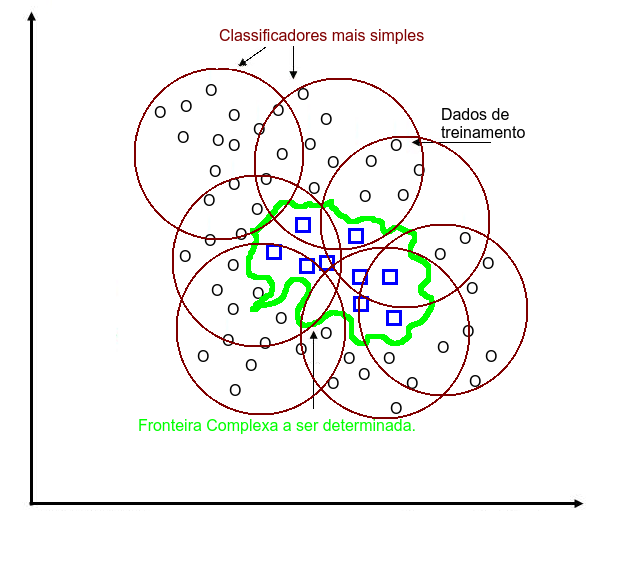
\includegraphics[width=8cm]{Imagens/Boost2.png}
\DeclareGraphicsExtensions.
\caption*{Fonte: Autor ``adaptado de'' \citefloat{Polikar}}
\label{Fig:Boost2}
\end{figure}


	\subsection{HAAR-Adaboost}

Somando-se todos os valores de cores de uma imagem, de forma que cada o valor em cada posição será a soma de todos os pixels acima e a esquerda daquela posição e armazenando esses valores em um vetor bidimensional, é possível calcular rapidamente o valor médio da cor em qualquer retângulo da imagem. Isso é feito subtraindo o valor encontrado no topo à esquerda do valor encontrado no fundo a direita e dividindo pelo número de pixels do retângulo. 

Segundo \citeonline{Xue}, outra particularidade dessa técnica é o tamanho da amostra. O tamanho da amostra se refere ao tamanho padrão de entrada dos classificadores de uma amostra de uma determinada imagem. As amostras são trechos retirados da imagem que possuem um determinado tamanho padrão. A imagem de origem é rotacionada aleatoriamente em volta de todos os eixos. Então pixels que possuem a intensidade dentro de um intervalo específico são interpretados como transparentes. Um ruído branco é adicionado às intensidades do plano de frente. A imagem obtida é então colocada dentro de um plano de fundo arbitrário proveniente do arquivo de descrição de fundos, redimensionada para a largura e altura desejados e então armazenadas em um vetor.

Muitos pesquisadores têm observado que adicionar mais classificadores fracos pode reduzir o erro de treinamento, mas dificilmente reduz o erro de generalização \cite{LiZhang} \cite{Brubaker} \cite{Mita}. Segundo \citeonline{Sakrapee} o desempenho da detecção decai drasticamente no estágios mais avançados da cascata, além disso, o desempenho da detecção usando características simples e únicas não são suficientemente discriminantes para separar imagens de faces das imagens onde faces não estão presentes. 

\citeonline{Mita} afirma que o uso da co-ocorrência de características em cada classificador fraco demonstrou um desempenho de classificação melhor do que se fossem utilizadas características simples. Assim, \citeonline{Sakrapee} propõe aplicar o conceito de unir características para criar a co-ocorrência de características. 

A contagem de amostras positivas \(N_{\text{AmostrasPositivas}}\) é um parâmetro muito importante, sem o qual o treinamento pode apresentar alguns erros ou pode nem mesmo prosseguir \cite{Mita}. Isso ocorre porque algumas amostras já utilizadas anteriormente por estágios já executados já podem ter sido classificadas isso pode manter o classificador em um mínimo local, a cada estágio a contagem de amostras positivas diminui até se tornar insuficiente. Para solucionar isso \citeonline{Maria} propôs o seguinte:

Suponha que um subconjunto de amostras positivas de tamanho \(N_{\text{AmostrasPositivas}}\) foi selecionado para treinar no estágio i, com i começando em zero, e \(Min_{\text{TaxaAcerto}}\) é a constante de treinamento para cada estágio.

Após treinar o estágio atual, pelo menos \(Min_{\text{TaxaAcerto}}\) * \(N_{\text{AmostrasPositivas}}\) amostras desse subconjunto devem passar por esse estágio, ou seja, o estágio atual da cascata com i+1 estágios tem que reconhecer a quantidade \(Min_{\text{TaxaAcerto}}\) das amostras selecionadas como positiva. Algumas amostras já utilizadas anteriormente por estágios já executados já podem ter sido classificadas como plano de fundo, mas não mais que ((1 - \(Min_{\text{TaxaAcerto}}\)) * \(N_{\text{AmostrasPositivas}}\)) em cada estágio. Veja equação ~\ref{eq1} onde, \(N_{\text{ImagensPositivas}}\) é a quantidade de imagens positivas total.

A equação ~\ref{eq2} foi usada para determinar o parâmetro \(N_{\text{AmostrasPositivas}}\).

\begin{equation}
\label{eq1} 
Amostras = ( N_{\text{Estágios}} - 1 ) * (1 - Min_{\text{TaxaAcerto}})
\end{equation} 

\begin{equation}
\label{eq2}
\begin{aligned}
N_{\text{ImagensPositivas}} = & [ N_{\text{AmostrasPositivas}} + Amostras * N_{\text{AmostrasPositivas}} ] + N_{\text{ImagensNegativas}} \\
			& \\
        		& \therefore  N_{\text{AmostrasPositivas}} = \frac { N_{\text{ImagensPositivas}} - N_{\text{ImagensNegativas}} } { 1 + Amostras} 
\end{aligned}
\end{equation}



A contagem de amostras do vetor que pode ser reconhecida como plano de fundo imediatamente é a variável \(N_{\text{ImagensNegativas}}\) na equação ~\ref{eq2}. 

\citeonline{Kuranov} afirmam que um tamanho de amostra de 20x20 pixels atingiu a maior taxa de acerto para detecção de faces. A cascata de classificadores foi implementada em formato de árvore, de forma que os ramos da árvore pudessem se dividir em 2 ou mais nós. \citeonline{Kuranov} afirmam também que para um tamanho de amostra de 18x18 e quatro nós de separação na fase de cascata tiveram um desempenho bom, enquanto para 20x20, dois nós a técnica teve um desempenho ligeiramente melhor, sendo a vantagem de desempenho entre usar 2, 3 ou 4 nós de separação nos classificadores fracos é menor do que a sua superioridade em relação a percorrer seus ramos. Sendo uma técnica usada para determinação de objetos o Haar-Adaboost será utilizado para identificar robôs da mesma forma que o HOG-SVM, de forma que uma comparação possa apontar qual deles se aplica nos robôs desenvolvidos.



\section{Controle Servo-Visual}

O controle servo-visual é uma técnica que usa o retorno de dados extraídos de um sensor de visão para controlar o movimento do robô. Esse tipo de controle, para o domínio RoboCup, se restringe ao controle dos dois servo-mecanismos referentes à cabeça do robô, mais especificamente do pescoço.

Uma das primeiras abordagens referentes ao controle servo-visual foi publicado por \citeonline{Corke}.Trabalhos mais recentes foram publicados por \citeonline{VS1} e por \citeonline{VS2}, aqui de uma forma mais abrangente no qual entende-se por controle servo-visual todas as ações feitas pelo robô que possuem como origem a visão do mesmo, inclusive movimentos das mãos, pés, rodas e articulações.

Técnicas de controle servo visual são classificados nos seguintes tipos:
\begin{enumerate}
     \item Baseada em Imagem (IBVS)
     \item Baseado Posição / Pose  (PBVS)
     \item Abordagem Híbrida
\end{enumerate}

A IBVS foi proposta por \citeonline{Weiss}. A lei de controle é baseada no erro entre as características atuais e desejadas no plano da imagem e não envolve qualquer estimativa da pose do alvo. Os recursos podem ser as coordenadas de recursos visuais, linhas ou momentos de regiões. A IBVS tem dificuldade com movimentos muito grandes, como rotações, o que veio a ser chamado retiro de câmera. \footnote{Do inglês: "Camera Retreat"}

A PBVS é uma técnica baseada em uma única câmera. Isto porque a posição do objeto de interesse é estimada em relação à câmera e, em seguida, é emitido um comando para o controlador de robô, que por sua vez, controla o robô. Neste caso, as características da imagem são extraídas mas, são, também, utilizadas para estimar a pose do objeto no espaço cartesiano.

Abordagens híbridas usam uma combinação dos controles previamente descritos. De forma geral, essas duas técnicas são consideradas passivas já que aguardam os dados do sensor de visão para tomar alguma decisão. 

Uma outra forma de encarar esse desafio é usar uma visão ativa, como proposta por \citeonline{Sharma}, que, de fato, procura ativamente o objeto a ser identificado e para tanto precisa tomar algumas decisões, mesmo que não haja dados relevantes vindos da câmera. 

Um sistema de visão ativo é capaz de interagir com o seu meio ambiente \cite{Tsotsos}, alterando o seu ponto de vista em vez de observá-lo passivamente e operando em sequências de imagens, em vez de em um único quadro \cite{Walther}. Além disso, a capacidade de acompanhar fisicamente um alvo reduz o borrão de movimento, aumentando a resolução de destino para tarefas de nível mais elevado, tais como classificação  \cite{Walther}. 

O controle servo-visual armazena as posições de trajetória do objeto e, por meio de regressão, estima as próximas posições do mesmo.  	Usando um algoritmo guloso encontra-se o melhor movimento antecipado da câmera em direção ao objeto. Para garantir um movimento plausível da câmera, é necessário considerar a cinemática e a dinâmica desse movimento, otimizando a trajetória da câmera para que essa possa manter o objeto em seu campo de visão.

Uma das vertentes da visão ativa é a configuração escravo-mestre \cite[p.2]{Fernandez}, no qual uma câmera está fixa e outra está em movimento. Ambas precisam estar em um mesmo sistema de coordenadas para que as informações trocadas entre elas sejam facilmente interpretadas. Essa configuração poderá ser usada em um projeto futuro, no qual o goleiro exerça o papel de câmera estática de supervisão enquanto os outros jogadores seriam as câmeras ativas em movimento. 

\section{Identificação de objetos}

% INTRODUÇÃO
Atualmente a visão computacional aplicada à robótica melhora no mesmo ritmo que a capacidade computacional. A quantidade de informação que uma imagem pode ser redundante ou desnecessária. Dessa forma o sistema de percepção deve reduzir ou tratar essa informação para que os objetivos sejam alcançados. 

Diversas abordagens têm sido propostas para o reconhecimento de objetos, sendo as mais recentes se valendo do uso de Redes Neurais Profundas (DNN) \cite{Deep1} \cite{Deep2} \cite{mccannobject}. A maioria usa uma ou mais características, geralmente únicas a esse objeto, fazendo-o sobressair aos demais itens na imagem capturada. Um ponto em comum às muitas das abordagens, decorre do uso de câmeras estáticas, nesse sentido o sistema poderia interpretar os dados provenientes da(s) câmera(s) de forma equivocada, já que a vibração da câmera causada pelo movimento do robô causa o borramento da região de interesse e arredores além de, provocar o movimento de pixels não pertencentes à essa região. 

Para reconhecer um objeto é necessário distinguí-lo do plano de fundo usando suas características únicas ou informação temporal, verificando quadro a quadro a região de interesse.

Com a finalidade de inferir algum formato à região de interesse, muitos algoritmos são propostos para a detecção de borda, incluindo o uso de gradientes. Reconhecer objetos parcialmente observáveis, em tempo real, torna-se uma tarefa particularmente difícil de  solucionar, já que um objeto parcialmente ocluso tem seu formato alterado. 

De forma análoga, a cor pode ser usada como uma forma de segmentar a região de interesse, que apesar de ser uma característica simples de se computar, é muito influenciada pela iluminação do ambiente. O time AUTMan, da Politécnica de Teerã \cite{AUTMan}, separa a imagem em três camadas, em cada qual segmenta uma cor referente à um objeto, sendo que cada uma dessas camadas serve de entrada para a próxima. Primeiramente as linhas de campo são segmentadas, em seguida o gol e por último, a bola. Dessa forma não é possível ver a bola se a segmentação do campo não estiver concluída. 

Todos os times participantes da Robocup são unânimes quanto ao uso de uma tabela de pesquisa (Look-up Table - LUT), na qual diversos valores de cor são armazenados previamente para uso na segmentação. Alguns times usam uma GUI (Graphical User Interface), Interface gráfica para Usuário para calibrar esses valores durante a competição.

\subsection{Reconhecimento da Bola}

Devido a importância da bola em jogo de futebol, o algoritmo de identificação da bola precisa ser rápido, robusto à oclusão e às diversas condições de iluminação. Algumas características da bola, como seu formato circular, sua cor e seu tamanho, são largamente utilizadas por todos os times, não só para encontrar a bola mas, também, para calcular sua distância do robô. 

%Como premissa, a bola apresentada em 2014 possuía cor predominantemente laranja, porém, devido ao seu polimento a mesma refletia uma certa quantidade de luz branca provenientes das luminárias.  

O filtro de Kalmann \cite{Kalmman} e o filtro de partículas proposto por \citeonline{AdaptPart}, também chamado de algoritmo de condensação  \cite{Condensation} para uso em imagens digitais, são amplamente usados em outros domínios como formas probabilísticas de inferir a posição de um objeto digital. São técnicas mais custosas em termos de tempo de computação mas, com mais poder de processamento, seria possível usá-las como uma forma complementar de identificar a posição na qual a bola se encontra.
 
Calcular a distância da bola ao robô, quando esta encontra-se parcialmente oclusa, adiciona uma componente de dificuldade, já que o tamanho conhecido da bola é usado como forma de computar essa distância. Nesse sentido, o time NUBots, da universidade de Newcastle \cite{Bunden}, criou linhas de varredura horizontais e verticais onde todos os pixels são considerados de forma individual. Determinam a linha de horizonte verde e, usando uma LUT, geram as transições referentes à classe de cor da bola. 

Esse mesmo time lidou com o problema da oclusão em 2012, adicionando uma etapa de verificação, onde quatro pontos de interesse, sem oclusão, podem ser usados em um método de atualização de centro, quando um determinado limite (threshold) de pixels consecutivos não pertencentes à bola são alcançados. Apesar de robusto contra ruído e alguma oclusão, esse método ainda precisa de duas verificações de tamanho e mais duas de cor. 

Esse algoritmo trabalha em baixo nível, segmentando pixels de forma individual e, por esse motivo, pode-se dizer que está efetuando a detecção com pouquíssimos recursos computacionais, infelizmente, trabalhando nesse nível, várias verificações precisam ser executadas de maneira que os pixels possam ser agrupados em regiões com uma mínima confiabilidade. A transformada de Hough probabilística usada pelo time Bold Hearts \citeonline{Bold}, da universidade de Hertfordshire, Inglaterra, parece fornecer essa confiabilidade ao custo de mais processamento. Nenhum time parece ter usado a informação temporal da câmera. Na verdade, o processamento aparenta ter sido efetuado como se tirassem diversas fotos e cada foto tivesse sido processada individualmente, sem que a informação do quadro anterior passasse para o próximo quadro.

Segmentar uma região por movimento é feito, de maneira geral, comparando os pixels do quadro atual com os pixels do quadro anterior, de forma individual ou em forma de máscaras. O rastreamento por fluxo ótico \cite{Fleet} funciona muito bem para câmeras estáticas onde os pixels que representam o plano de fundo tem pouca ou nenhuma alteração são facilmente subtraídos, deixando apenas os pixels que podem significar um objeto em movimento. Para o robô proposto, a câmera se movimenta e oscila frequentemente fazendo com que essa técnica apresente regiões provenientes de falsos movimentos, visto que, se a câmera inteira se mover muitos pixels que deveriam ser considerados parte do plano de fundo se moverão também.


\subsection{Identificação dos Robôs}
% RECONHECIMENTO DOS ROBÔS

Um importante item de um jogador de futebol é saber se seu adversário está a caminho de roubar-lhe a bola, ou saber a posição de seu companheiro de equipe para efetuar um passe. A identificação de robôs é especialmente difícil já que a variedade de robôs da liga é grande e a cada ano esses são modificados por suas equipes. Na verdade, na liga nenhum time demonstrou em seu trabalho de descrição de times qualquer menção ao reconhecimento de robôs.

O maior problema do algoritmo de reconhecimento de robôs é executá-lo em tempo real, devido ao número de dimensões ou características dos robôs e do fundo serem consideravelmente elevados, assim como, seus custos computacionais. Devido ao exposto, deve haver uma redução de características menos importantes. Na verdade o problema de reconhecimento dos robôs pode ser dividido em três partes:

\begin{itemize}
\item{Redução de características com a extração dos descritores mais relevantes;}
\item{Treinamento e classificação (É robô ou não é robô);}
\item{Identificação do time pela sua respectiva cor. (Sorteada no começo da partida)}
\end{itemize}

Um dos mais populares e bem sucedidos detectores de pessoas é o Histograma de Gradientes Orientados  \footnote{HOG - Do inglês: "Histogram of Oriented Gradients"}, usado juntamente com o classificador Máquina de Vetores de Suporte \footnote{SVM - Do inglês: "Support Vector Machine"}.

\citeonline{Castro} utilizaram essa abordagem com uma segmentação de cores para identificar a qual time cada robô pertence após um reconhecimento do torso do robô NAO \cite{NAO}\footnote{TDP - Do inglês: "Team Description Papers"}. Na standard platform league, todos os robôs obedecem ao padrão NAO, portanto se faz necessário identificar apenas um robô, e todos os outros terão o mesmo formato. Decorre do treinamento mais um problema dessa aplicação, a variedade de robôs presentes na categoria KidSize pode dificultar esse objetivo.

Há outros algoritmos que poderiam ser usados, como o Centrist \cite{Wu}. Outros detectores usam o movimento para iniciar o rastreamento e, como já foi visto, a câmera na cabeça do robô vibra muito. Outros classificadores como o LBP \cite{Viola}, o PCA/LDA \cite{Martinez}, entre outros, podem ser usados já que a classificação ocorre comparando vetores de descritores de treinamento com vetores de teste.

\begin{table}[ht!]
    \caption{Quadro de referência} \label{tbl:Times}
    \centering
    \begin{tabular}{|c|c|c|c|c|c|c|}
    \hline 
    Time 	& Sistema 	& Segmen  	& Bola		& Gol 		   & Linhas	   & Robô	\\ 
    	 	& Cores   	& tação		& 		&     		   & Campo	   & 	 	\\ 
    \hline 

    CIT 	& RGB - HSV 	& LUT	  	& Transição	&  Transição	   & Segmentação   & --	     	\\
    Brains	& 	 	& 	  	& de pixels	&  de pixels	   & Branco com    &	     	\\
    		& 	 	& 	  	& 		&  	 	   & Verificação   &	     	\\
    		& 	 	& 	  	& 		&  	 	   & Linear        &	     	\\

    \hline 

    Bold 	& RGB - HSV 	& LUT	  	& Transição	&  Transformada	   & Segmentação   & --     	\\
    Hearts	& 	 	& 	  	& de pixels	&  Hough 	   & Branco e      &	     	\\
    		& 	 	& 	  	& 		&  Probabi-  	   & Regressão     &	     	\\
    		& 	 	& 	  	& 		&  -lística	   & Linear        &	     	\\
    \hline 

    Baset	& RGB - HSV 	& LUT	  	& Transição	&  Transição	   & Segmentação   &            \\
    		& 	 	& 	  	& de pixels	&  de pixels	   & Branco        & --     	\\
    		& 	 	& 	  	& Contornos	&  Contornos       & RANSAC        &	     	\\
    \hline 

    Eros	& YUYV  	& LUT	  	& Transição	&  Transformada	   & Segmentação   & --	     	\\
    		& nativo	& 	  	& de pixels	&  de Hough	   & Branco        &	     	\\

    \hline 
     
    AUTMan	& RGB - HSV 	& LUT	  	& Transição	&  Transição	   & Segmentação   & --	     \\
    		& 	 	& 	  	& de pixels	&  de pixels       & Branco        &	     \\
    \hline

    \end{tabular}
    \caption*{Fonte: Artigos de Descrição de Equipes$^4$, 2014 \cite{AUTMan}, \cite{Bold}, \cite{CIT}, \cite{Baset}, \cite{EROS} }

\end{table}

\section{Considerações finais}

Vimos nesse capítulo que as equipes, inseridas no domínio RoboCup, trabalham em baixo nível e em médio nível \cite{AUTMan}, \cite{Bold}, \cite{CIT}, \cite{Baset}, \cite{EROS}. Essas técnicas são bem utilizadas e têm resultados pertinentes porém, com a mudança das regras, esses algoritmos vão precisar de cada vez mais estágios de verificação. Vimos também que diversas adversidades são inerentes do domínio, e que por esse motivo precisam de técnicas que possam identificar características, mas, que também, possam levar em conta algum contexto do objeto pertencente ao jogo.
Dessa forma, ao lançar o artifício de utilizar técnicas de alto nível e considerando o que outras equipes têm feito, serão abordados no próximo capítulo dois aspectos do sistema de visão: 

\begin{enumerate}
	\item a identificação e rastreamento da bola.
		\begin{enumerate}
			\item Algoritmo proposto conforme algoritimo ~\ref{lst:algBall}
			\item Descritor e Classificador Haar-AdaBoost
		\end{enumerate}
	\item a detecção de robôs.
		\begin{enumerate}
			\item Descritor e Classificador HOG-SVM
			\item Descritor e Classificador Haar-AdaBoost
		\end{enumerate}
\end{enumerate}

Nos dois casos, as técnicas serão postas a prova com o mesmo conjunto de imagens pertinentes aos seus respectivos objetivos. De maneira que possam coexistir no sistema de visão do robô sem onerá-lo em demasia.





